
\chapter{System w~użyciu}
\label{sec:Praktyka}

\section{Uruchomienie Inkubatora}
Inkubator powinien stać w~pomieszczeniu w~miejscu przewiewnym i~suchym. Przed
uruchomieniem Inkubatora należy dokładnie wymyć komorę inkubacyjną. W~tym celu
można wyciągnąć z~komory ramki z~rolkami i~przemyć ściany komory płynem
dezynfekującym. Ponadto należy uzupełnić pojemnik z~wodą destylowaną do
nawilżania powietrza. Po tych czynnościach można podłączyć Inkubator do
zasilania oraz sieci lokalnej Ethernet i~uruchomić go. Inkubator uruchamia się
około 2~minut, w~tym czasie ładowany jest do pamięci system operacyjny
i~uruchamiana jest aplikacja sterująca. Po uruchomieniu na ekranie
inkubatora pojawi się odpowiedni komunikat. Jeżeli przed ostatnim wyłączeniem
inkubator znajdował się w~trakcie inkubacji to automatycznie przystąpi on do
kontynuowania tego procesu i~sterowania nim. Jeżeli natomiast jest to pierwsze
uruchomienie lub poprzednia inkubacja została zakończona, Inkubator będzie
gotowy do zaprogramowania nowej inkubacji. Do zaprogramowania można wykorzystać
Stację Kontrolną lub wbudowaną klawiaturę.

\section{Programowanie Inkubatora przy użyciu wbudowanej klawiatury}
Po uruchomieniu Inkubatora użytkownik może wybrać z~menu aplikacji rozpoczęcie
nowej inkubacji lub modyfikację trwającego procesu. W~obu przypadkach
programowanie polega na podaniu punktów, przez które ma przebiegać zadana
funkcja temperatury i~wilgotności. Do zdefiniowania każdego punktu należy podać
chwilę czasu oraz zadaną wartość sterowanego parametru w~tej chwili.
W~minimalnej wersji do zaprogramowania przebiegu temperatury wystarczy podać
2~punkty: pożądaną temperaturę w~momencie rozpoczęcia inkubacji oraz w~momencie
zakończenia. Algorytm sterowania połączy podane punkty linią łamaną tworząc zadaną
funkcję sterowanego parametru. Podczas programowania należy również podać
częstość obracania jaj i~wychładzania inkubatora.

\section{Stacja Kontrolna}
Wykorzystanie Stacji Kontrolnej wymaga, aby inkubatory oraz Stacja Kontrolna
znajdowały się w~jednej sieci lokalnej. Podczas uruchomienia aplikacja Stacja
Kontrolna automatycznie wyszukuje znajdujące się w~sieci Inkubatory i~rozpoczyna
zbieranie pomiarów.

\subsection{Interfejs kontroli}
Po uruchomieniu aplikacji Stacja Kontrolna otwarte jest okno kontroli
(ControlWindow) przedstawione na rysunku \ref{rys:Control}. Na górnym panelu
wyświetlone są panele monitorujące poszczególne inkubatory. Przedstawiają one
wykres temperatury i~wilgotności w~funkcji czasu z~ostatniej doby. Aby uzyskać
szczegółowe informacje o~którymś inkubatorze należy kliknąć na monitorujący go
panel. W~lewym panelu wyświetlana jest wówczas informacja o~gatunkach ptaków,
których jaja znajdują się w~wybranym inkubatorze. Pozostałą cześć okna zajmuje
wykres szczegółowy temperatury i~wilgotności w~wybranym inkubatorze. Na osi
poziomej odłożono czas, zaś na osi pionowej wartość temperatury i~wilgotności.
Wykres szczegółowy można dowolnie przesuwać wzdłuż wszystkich osi oraz robić
dowolne zbliżenia przy pomocy urządzenia wskazującego. Dla ułatwienia nawigacji
po wykresie pod prawym przyciskiem myszy dostępnych jest kilka opcji
automatycznego doboru rozmiaru wykresu. Na wykresie oprócz faktycznych wartości
temperatury i~wilgotności nanoszone są również wartości zaplanowane. Pozwala to
sprawdzić czy dana inkubacja przebiega zgodnie z~planem od momentu rozpoczęcia.
Wszystkie dane pomiarowe są automatycznie zapisywane na dysku. Dzięki temu po
ponownym uruchomieniu aplikacji nie trzeba pobierać starych pomiarów
z~inkubatora.

\begin{figure}[p] 
\centering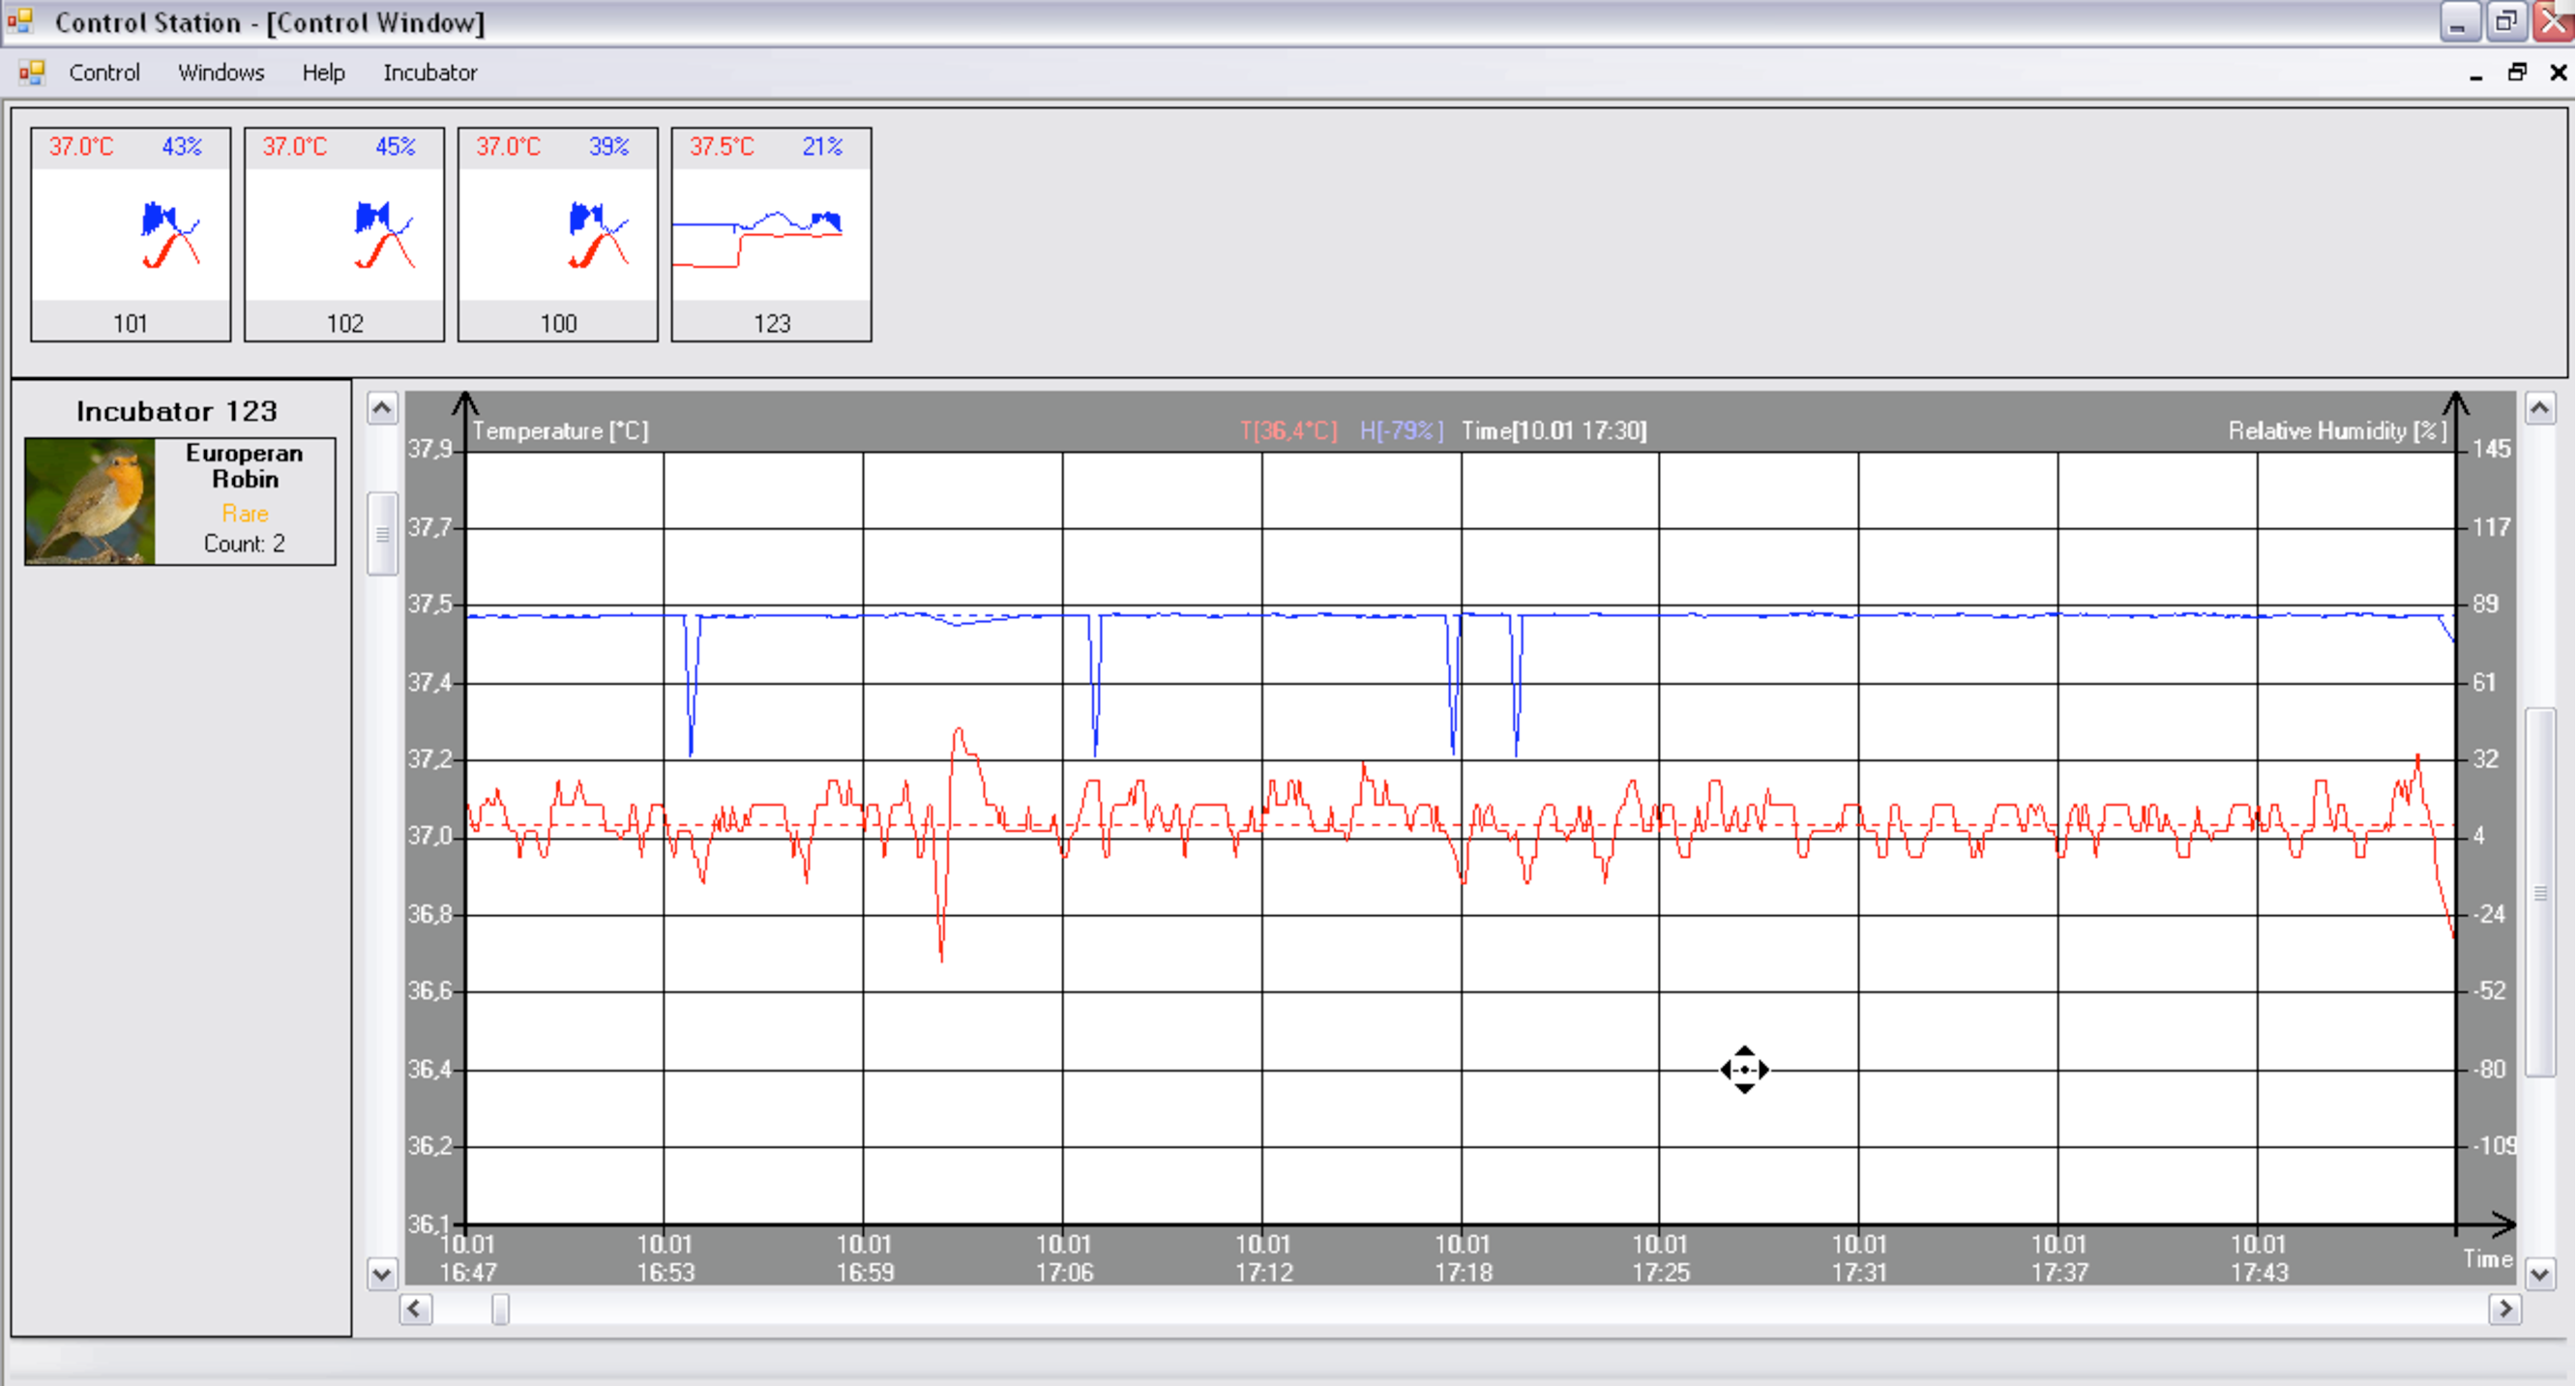
\includegraphics[width=\textwidth]{figures/Control}
\caption{Okno kontroli}\label{rys:Control}
\end{figure}

\begin{figure}[p] 
\centering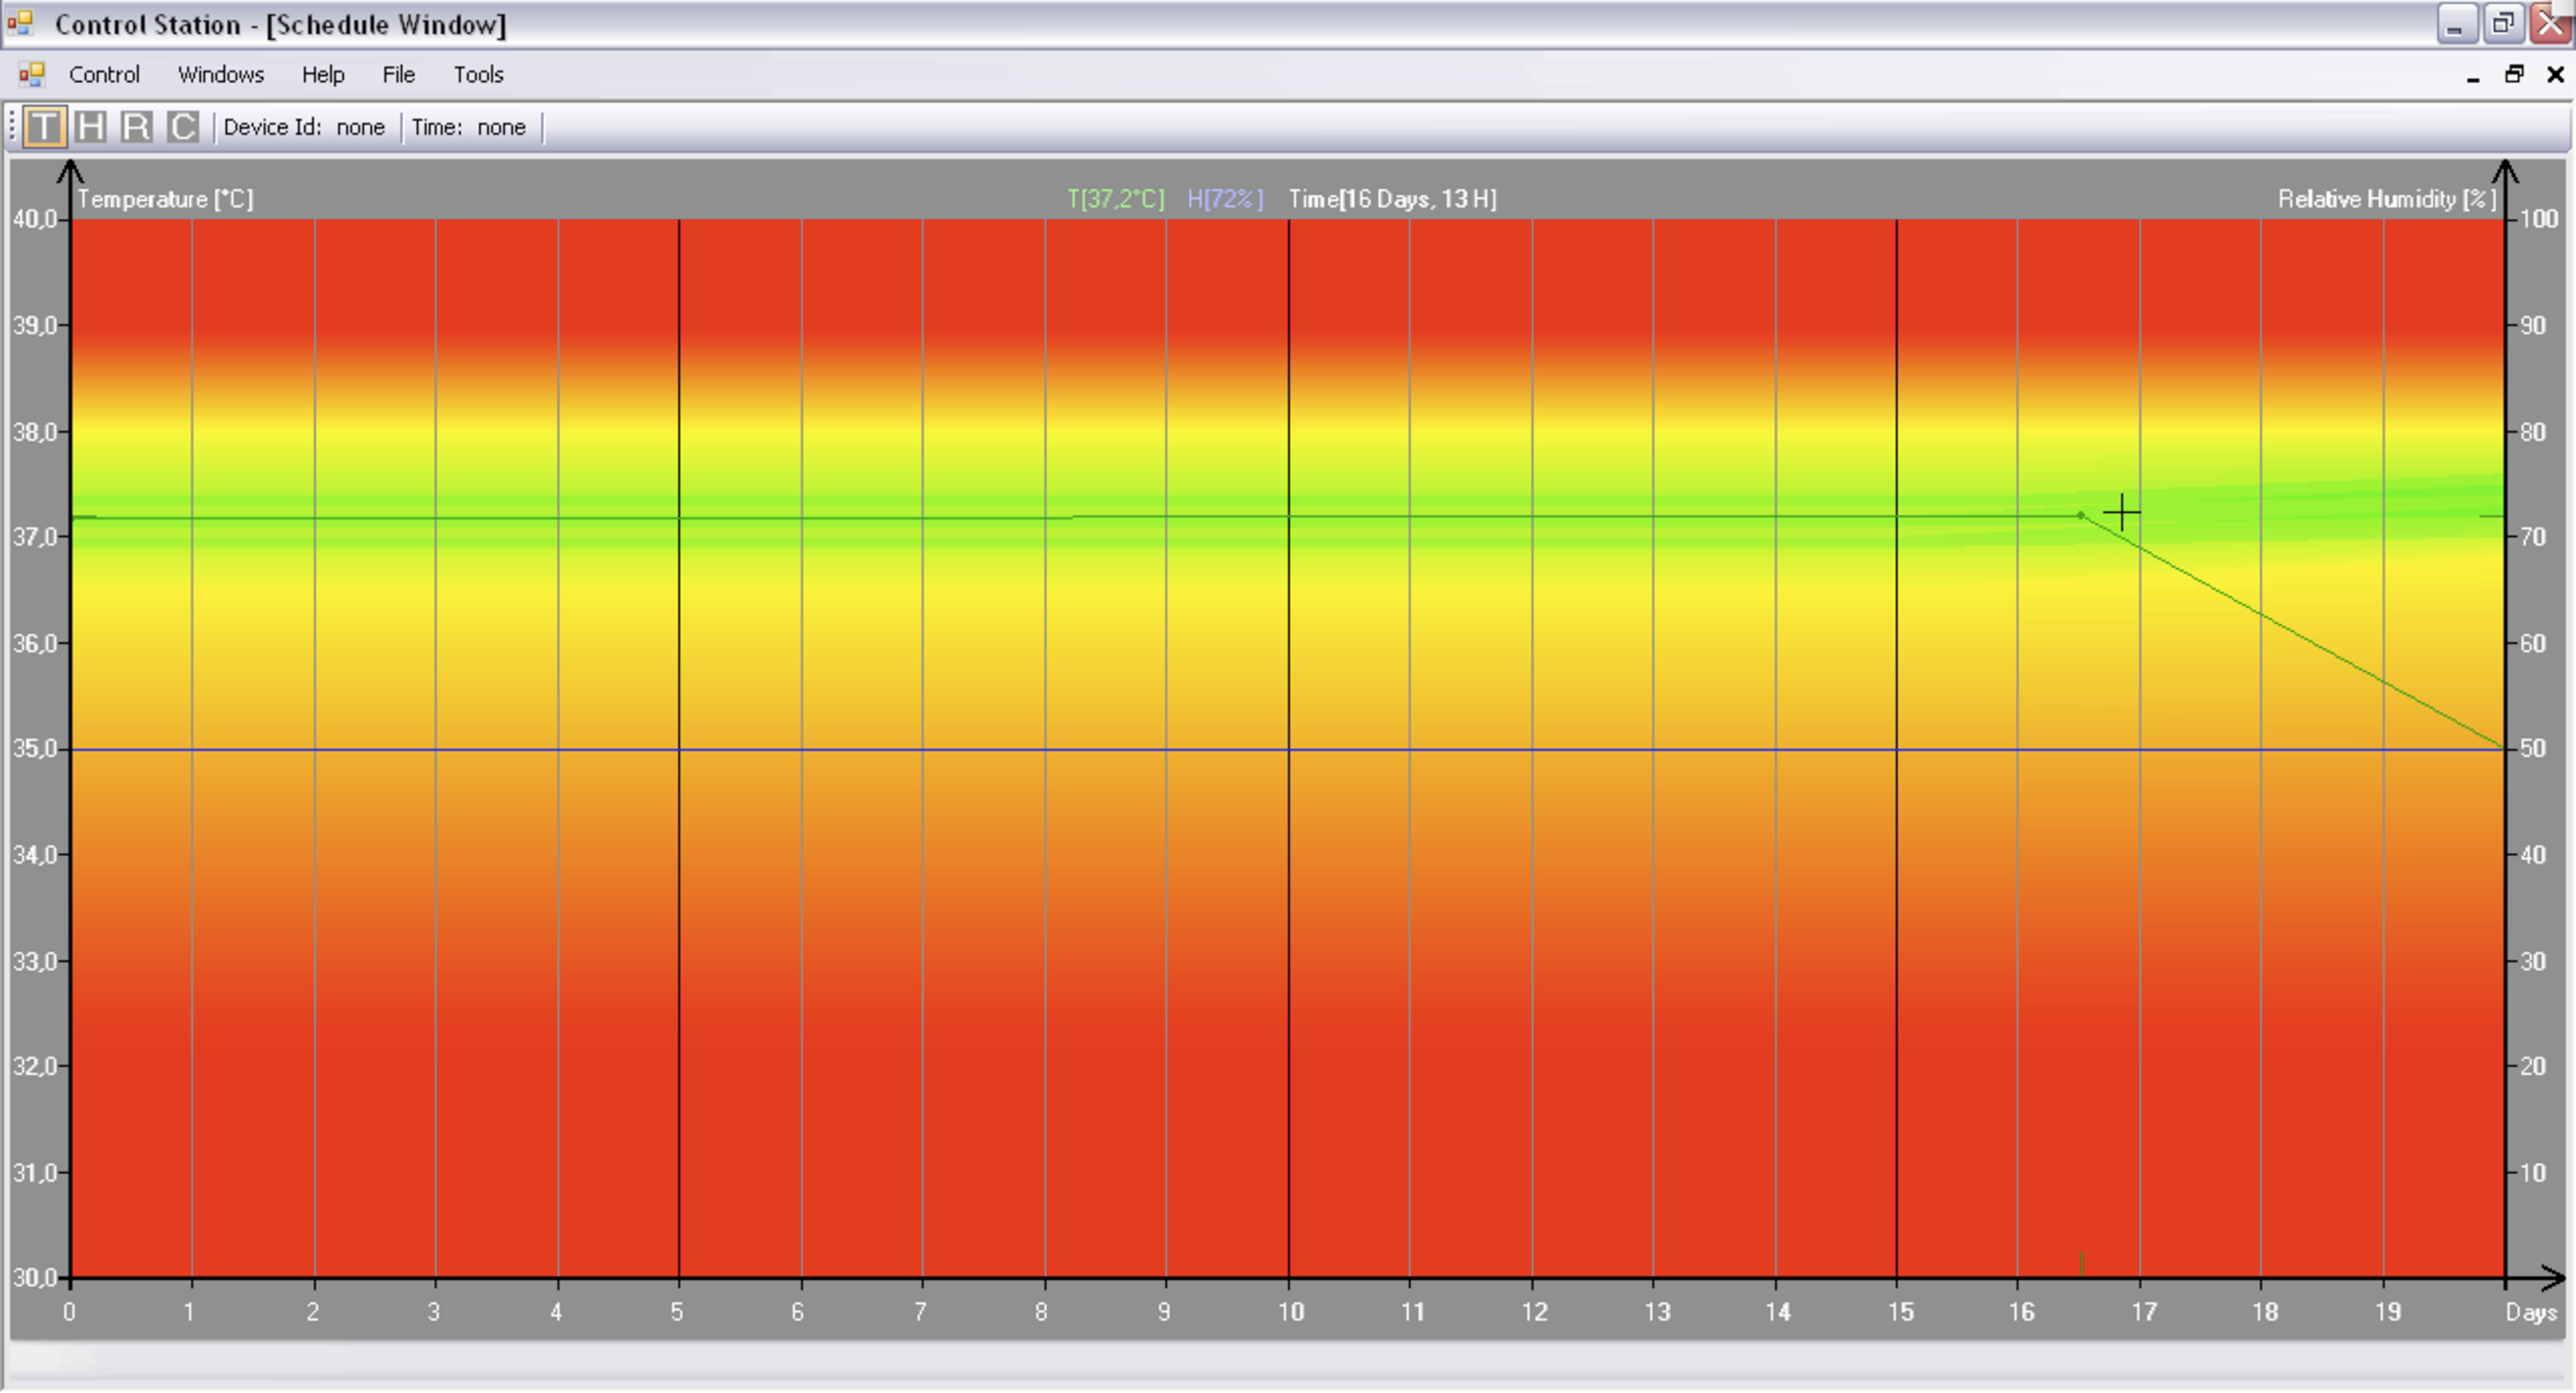
\includegraphics[width=\textwidth]{figures/Schedule}
\caption{Okno Planu Inkubacji z~nałożonymi na siebie wzorcami inkubacji trzech różnych gatunków}\label{rys:Schedule}
\end{figure}

\subsection{Interfejs programowania}
Po wyborze w~menu opcji ,,Schedule'' (Plan inkubacji) wyświetlane jest okno
programowania (ScheduleWindow) przedstawione na rysunku~\ref{rys:Schedule}. Okno
to służy do ustalenia pożądanych wartości sterowanych parametrów inkubacji. Na
pasku narzędzi do wyboru jest temperatura, wilgotność oraz częstość obracania
i~chłodzenia. Ustalanie przebiegu funkcji sterowanych parametrów odbywa się
podobnie jak w~inkubatorze przez dobór punktów (czas, wartość) przez które ma
przebiegać zadana funkcja. Użytkownik może też określić gatunki ptaków, których
jaja chce inkubować, wybierając z~menu opcję ,,Tools'' (Narzędzia) $\rightarrow$
,,Species'' (Gatunki). Okno dialogowe wyboru gatunków przedstawione jest na
rysunku~\ref{rys:Species}. Po wyborze gatunków w~tle wykresu pojawiają się
nałożone na siebie wzorce inkubacji wybranych gatunków. Mają one postać
gradientu koloru od czerwonego (dla zbyt wysokich wartości), poprzez zielony
(dla optymalnych wartości) do czerwonego (dla zbyt niskich wartości ustalanej
funkcji). Użytkownik powinien tak ustalać przebieg funkcji by znajdowała się ona
w obszarze optymalnym. Na wspomnianym rysunku~\ref{rys:Schedule} nałożone są
wzorce temperatury dla trzech różnych gatunków. Jak widać obszary optymalne dla
wybranych gatunków przesunięte są względem siebie o~około~0,2\st. Zielona
pozioma kreska przedstawia przebieg funkcji temperatury, dobrany tak by
minimalizować łączny błąd nastaw względem wzorca. Po ustaleniu wszystkich
parametrów plan inkubacji można przesłać do inkubatora. W~tym celu należy wybrać
w~menu opcję ,,Tools'' (Narzędzia) $\rightarrow$ ,,Send schedule'' (Prześlij
plan inkubacji). Pojawia się wówczas okno dialogowe
(rysunek~\ref{rys:SendSchedule}), w~którym użytkownik wybiera identyfikator
inkubatora, który chce zaprogramować. Wybrany inkubator otrzymuje nowy plan
inkubacji i~od tej chwili zaczyna go realizować.

\begin{figure}[b]
	\centering
	\subfloat[Wybór inkubowanych gatunków]{
		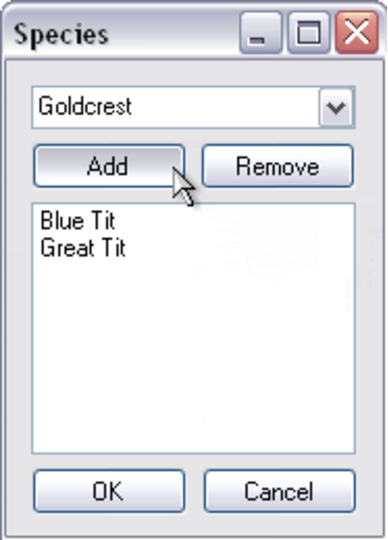
\includegraphics[width=0.3\textwidth]{figures/Species}
		\label{rys:Species}
	}
	\hfill
	\subfloat[Wysyłanie planu inkubacji do inkubatora]{
		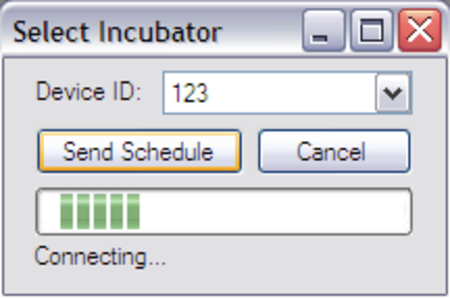
\includegraphics[width=0.3\textwidth]{figures/SendSchedule}
		\label{rys:SendSchedule}
	}
	\hfill
	\subfloat[Pobieranie planu inkubacji od inkubatora]{
		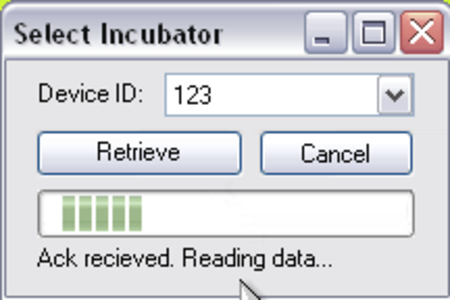
\includegraphics[width=0.3\textwidth]{figures/Retrieve}
		\label{rys:Retrieve}
	}

	\caption{Okna dialogowe w~Stacji Kontrolnej}
	\label{rys:dialogi}
\end{figure}

Okno programowania (ScheduleWindow) pozwala też na pobranie z~inkubatora
aktualnego planu inkubacji. W~tym celu należy wybrać z~menu opcję ,,Tools''
(Narzędzia) $\rightarrow$ ,,Retrieve schedule'' (Pobierz plan inkubacji).
Podobnie jak przy wysyłaniu, w~oknie dialogowym (rysunek \ref{rys:Retrieve})
należy podać identyfikator inkubatora, z~którego ma być pobrany plan inkubacji.
Pobrany plan można dowolnie zmodyfikować i~przesłać z~powrotem do inkubatora.

\section{Centrum Nadzoru}

\subsection{Strona wstępu}
Na tej stronie użytkownik może zobaczyć informacje o~projekcie. Można tutaj
zamieścić informacje ułatwiające użytkownikowi korzystanie z~systemu
(\emph{FAQ} -- często zadawane pytania lub \emph{HOWTO} -- poradnik)
% tu bedzie obrazek

\subsection{Strona inkubacji}
Na tej stronie użytkownik może obejrzeć stan inkubacji (takiej, która się toczy
lub takiej która się zakończyła), którą może wybrać z~menu po lewej stronie.
W~górnej liście zakładek może zobaczyć informację odnośnie liczby inkubowanych
jaj lub wyklutych piskląt w~danej inkubacji. Na każdej zakładce dostępne są
informacje o~innym gatunku. W~dolnej liście zakładek użytkownik może zobaczyć
wykres reprezentujący stan zmiennych procesowych w~czasie. W~każdej zakładce
dostępne są informację o~innej zmiennej.
% tu bedzie obrazek

\subsection{Strona inkubatora}
Na tej stronie (rysunek~\ref{rys:CNinkubator}) użytkownik może przejrzeć stan inkubatorów w~jego grupie -- lista
dostępnych inkubatorów jest dostępna w~lewej części strony. Może również
ustawić czas, po którym zostanie do niego wysłany e-mail alarmujący,
gdy Centrum Nadzoru nie uzyska informacji o~stanie inkubatora.
% tu bedzie obrazek

\subsection{Strona gatunku}
Na tej stronie (rysunek~\ref{rys:CNgatunek}) użytkownik może zobaczyć obrazek przedstawiciela gatunku, krótką
informację oraz statystyki opisujące stan wiedzy systemu na temat tego gatunku
(np. ilość inkubacji, średnia klujność). Najciekawszą informacją na tej stronie
jest wzorzec inkubacji dla danego gatunku. Ze względów bezpieczeństwa użytkownik
nie może edytować stałych używanych przy generowaniu wzorców, może je jedynie obejrzeć.

\begin{figure}[p] 
\centering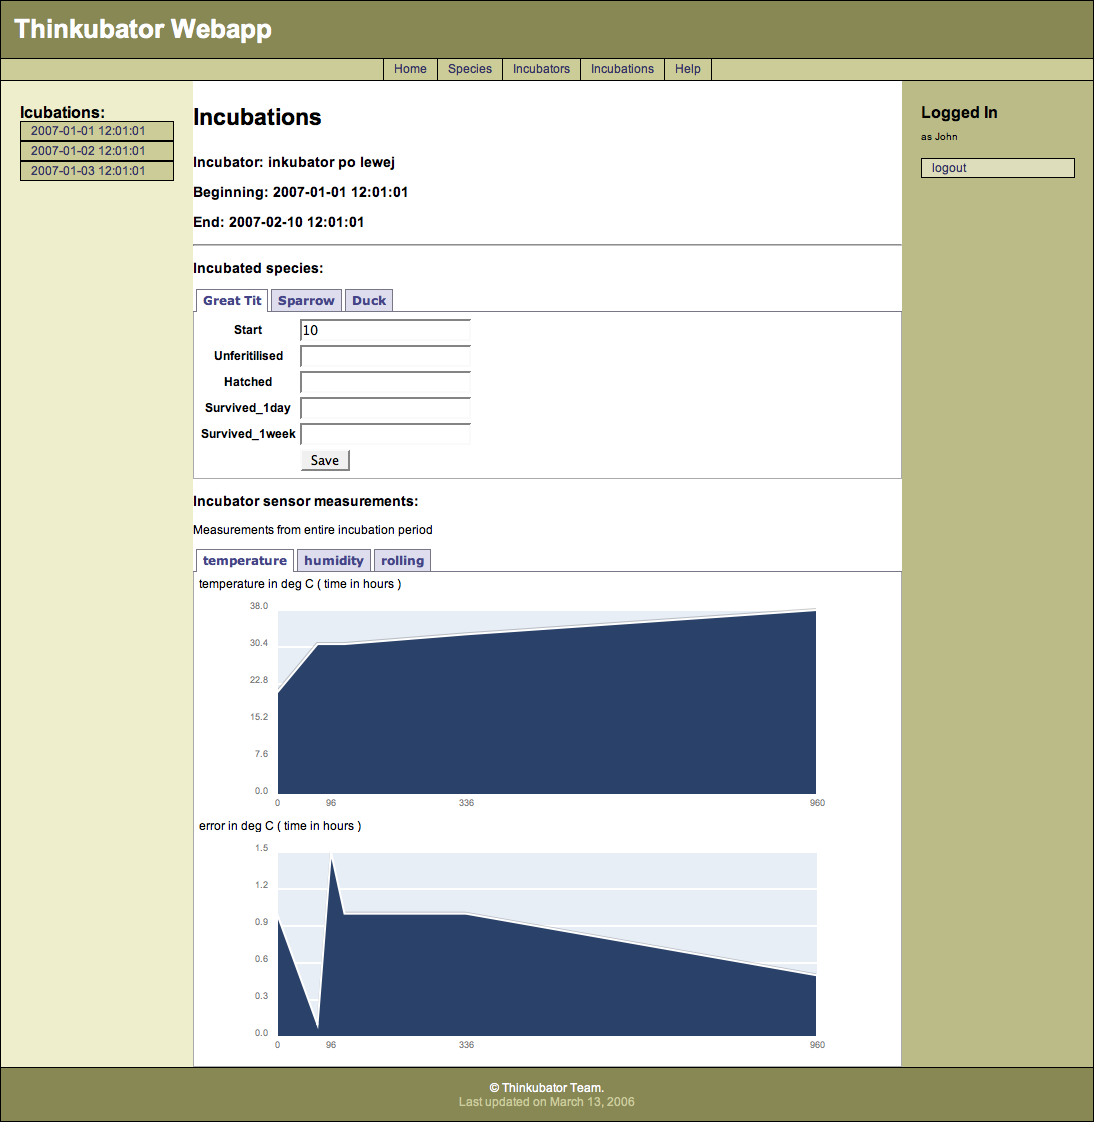
\includegraphics[width=.8\textwidth]{figures/CNinkubator}
\caption{Strona inkubatora}\label{rys:CNinkubator}
\end{figure}

\begin{figure}[p] 
\centering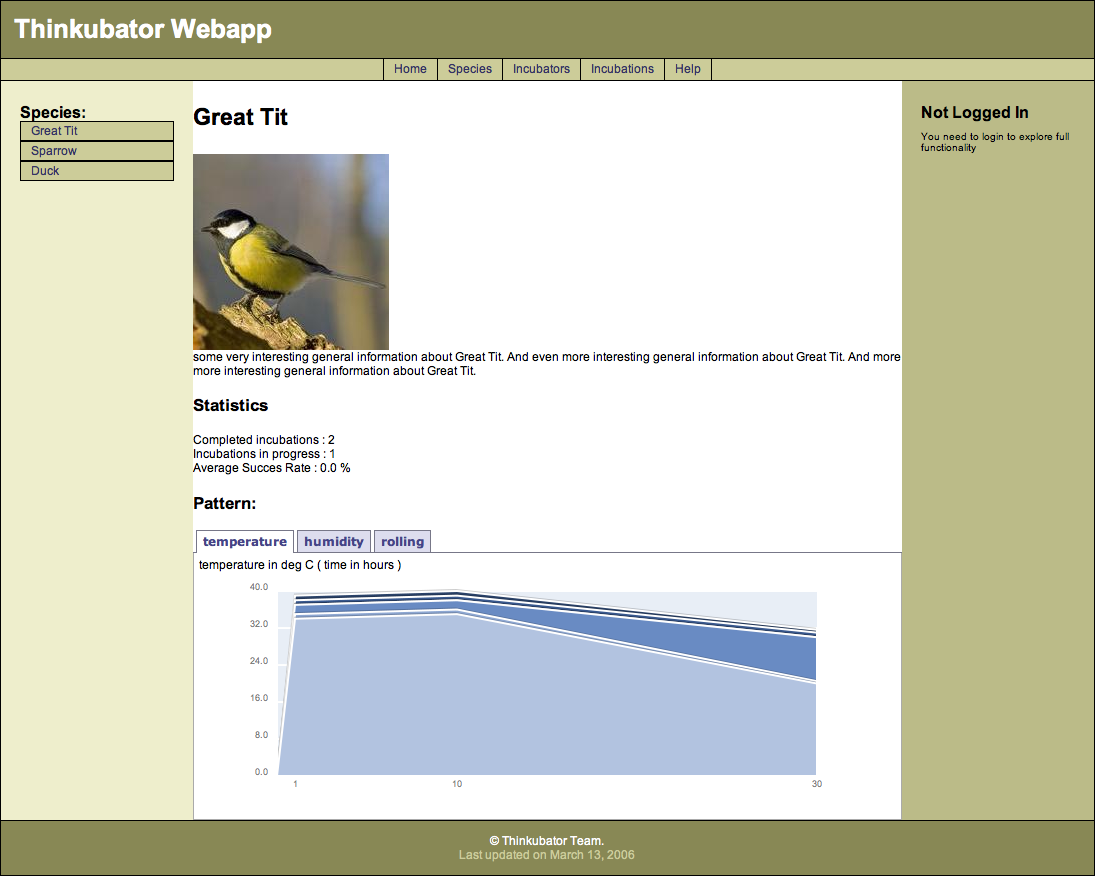
\includegraphics[width=.8\textwidth]{figures/CNgatunek}
\caption{Strona gatunku}\label{rys:CNgatunek}
\end{figure}

\subsection{Interfejs administracyjny}
Na tej stronie Administrator może bezpośrednio edytować zawartość bazy danych.
Dzięki temu ma on ułatwiony dostęp do jej zawartości i~może wygodnie edytować
wartości, które mają wpływ na globalną pracę systemu. Może on również poprawiać
błędy użytkowników.
% tu będzie obrazek

